\chapter{Research and design approach} \label{research_and_design_approach} \todo{<<DIT HOODSTUK MOET NOG VOLLEDIG WORDEN AANGEPAST>>}



This chapter describes the overall research design approach and contains the conceptual
framework that is applicable for research assignment at hand. 

\section{Research model}
The research approach is based on the Design Science method. The following section
describes the research model based on the Design Science research framework \parencite[(P.
107)]{recker_scientific_2013}. According to \citeauthor{recker_scientific_2013} Design
Science has been formulated as followed:

\begin{center}
    \enquote*{\textit{A research paradigm in which a designer answers questions relevant
    to human problems via the creation of innovative artifacts, thereby contributing new
    knowledge to the body of scientific evidence. The designed artifacts are both useful
    and fundamental in understanding that problem.}}
\end{center}
Figure \ref{fig:reserach_approach} depicts a graphical view of the research approach based
on the Design Science Research framework. The fundamental components of this research are
two separate artifacts. 

\begin{figure}[!h]
    \centering
    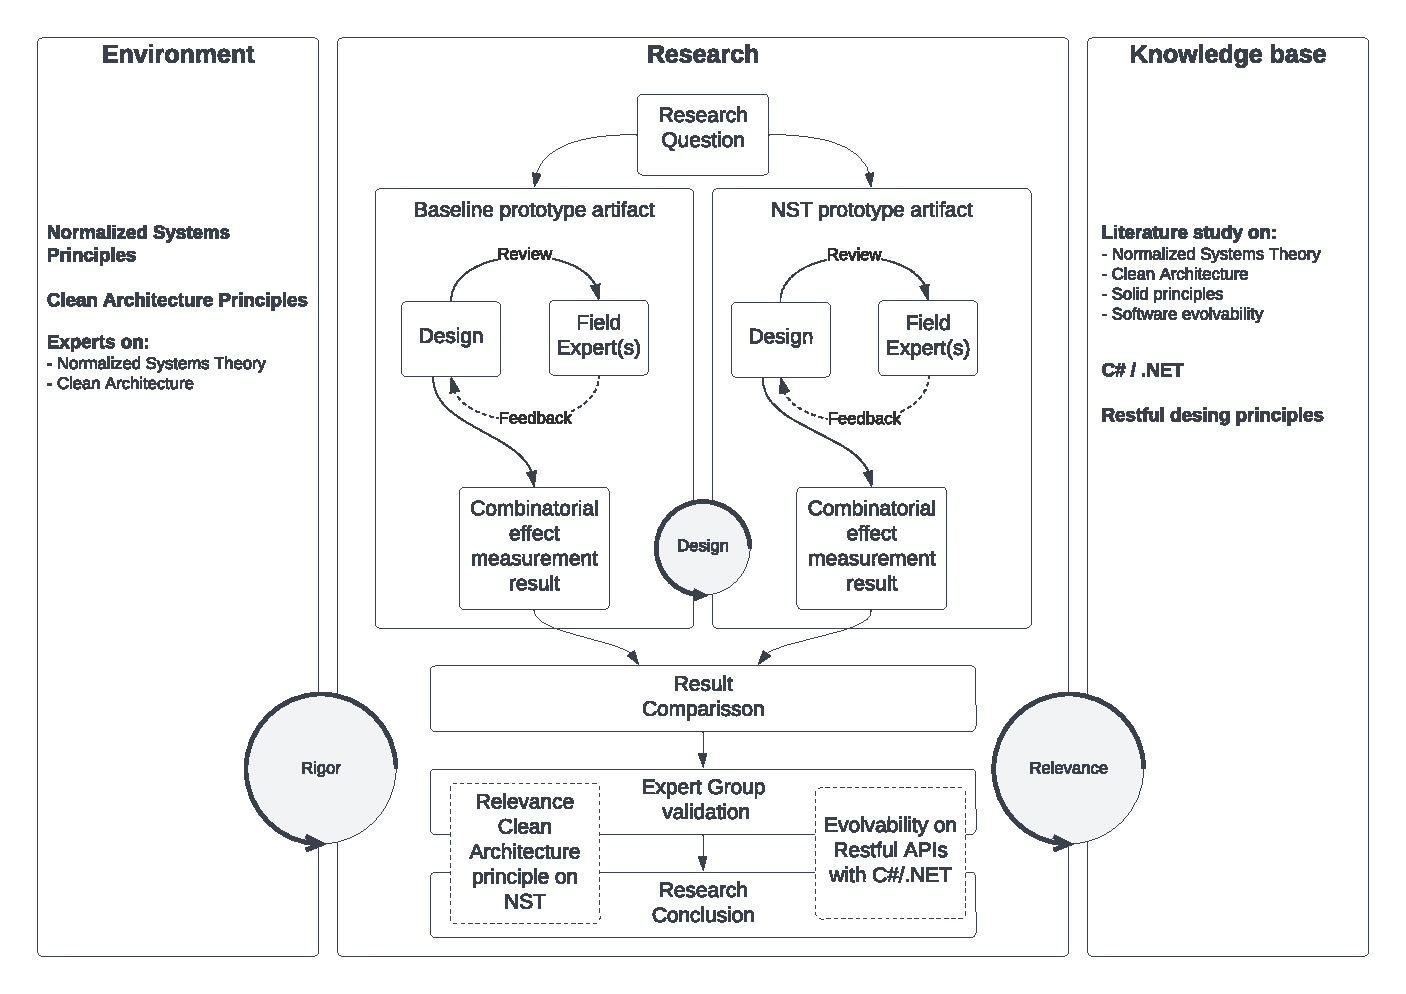
\includegraphics[width=1\textwidth]{Figures/research_approach}
    \caption[Research approach]{Research approach.}
    \label{fig:reserach_approach}
\end{figure}

The first artifact is intended to be a working prototype of a Restful API, designed
following to the Clean Architecture principles \parencite[]{martin_clean_2018} using
C\#/.NET programming language. The second artifact follows the results of the baseline
artifact. It is enhanced with the design based on the Normalized Systems Theorems. The
artifact uses the Software Generation concepts like expanding, rejuvenation and harvesting
as proposed in the paper \enquote{\citefield[]{mannaert_realization_2020}{title}}
\parencite[]{mannaert_realization_2020}

Each artifact will endure a review cycle done by field experts of on each of the given
design principles. The review cycle is used to ensure that the design and implementation
are according to those design principles.

Besides the review of the field experts, the artifacts will also be validated by using an automated
instrument (script) that measures the number of combinatorial effects on both of the
artifacts. The combinatorial effects are measured in a spectrum of changes in different
area's of the artifacts. For example:
\begin{itemize}
    \item {A change in a data entity}
    \item {A change in a use case}
    \item {A change in an action}
    \item {A change in a validation}
    \item {etc...}
\end{itemize}

The outcome of the measurements on combinatorial effects on both artifacts are the basis
for the comparison results. These results will be discussed and validated by a control
group determining the effect on the evolvability when using the Normalized Systems
Theorems in a C\#/.NET restful API. 
